\documentclass[]{article}

\usepackage{arxiv}
\usepackage[utf8]{inputenc} % allow utf-8 input
\usepackage[T1]{fontenc}    % use 8-bit T1 fonts
\usepackage{hyperref}       % hyperlinks
\usepackage{url}            % simple URL typesetting
\usepackage{booktabs}       % professional-quality tables
\usepackage{amsfonts}       % blackboard math symbols
\usepackage{nicefrac}       % compact symbols for 1/2, etc.
\usepackage{microtype}      % microtypography
\usepackage{lipsum}
\usepackage{graphicx}	% Including figure files
\usepackage{mathtools}  %loads amsmath as well
\usepackage{amssymb}	% Extra maths symbols
\usepackage[english]{babel}
\usepackage{float}
\usepackage{bm}
\usepackage{indentfirst}
\usepackage{tikz}
\usetikzlibrary{positioning}
\usepackage{pgfplots}
\usepackage{color,soul}
%\pgfplotsset{compat=1.12}
\definecolor{mygray}{RGB}{125,125,125}
\definecolor{myred}{RGB}{255,60,60}
\definecolor{myblue}{RGB}{60,60,255}
\renewcommand{\arraystretch}{1.2}

% potential journals:
    % journal of computational physics
    % computers and fluids
    % international journal for numerical methods in fluids
    % aiaa
    % journal of fluid mechanics


\title{A multiresolution scheme for adaptive computations on block-structured AMR meshes: applications to reactive flows}

\author{
  Brandon Gusto\\
  Department of Scientific Computing\\
  Florida State University\\
  Tallahassee, FL 32306 \\
  \texttt{bgusto@fsu.edu} \\
  %% examples of more authors
  \And
  Tomasz Plewa \\
  Department of Scientific Computing\\
  Florida State University\\
  Tallahassee, FL 32306 \\
  \texttt{tplewa@fsu.edu} \\
}

\begin{document}
\maketitle

\begin{abstract}
    We present a novel block-structured adaptive mesh refinement scheme
    featuring fully adaptive calculation of fluxes and source terms. The scheme
    addresses a major shortcoming of tree-based AMR codes: that the graded
    nature of the AMR mesh yields blocks whose cells are resolved beyond the
    desired error tolerance. To overcome this issue, we introduce a
    multiresolution representation of the solution not only for the purpose of
    grid adaptation but also to identify regions where fluxes and
    reaction-driven source terms can be interpolated from coarser levels. The
    error introduced by this approximation procedure is shown to be of the same
    order as the local truncation error of the reconstruction scheme. Thus the
    rate of convergence of the underlying spatial reconstruction scheme is
    preserved.  Additionally with respect to parallel applications, the
    multiresolution transform and computation of fluxes and sources on adaptive
    blocks is asynchronous, requiring only one synchronization step which is
    equivalent to the filling of ghost cells for each block. The efficiency of
    the scheme is demonstrated for problems in compressible flow and
    reaction-driven combustion.
\end{abstract}

% keywords can be removed
\keywords{multiresolution \and adaptive mesh refinement \and reactive flows}

\section{Introduction}

    % paragraph introduces the need for spatially adaptive grids
    Energetic, reacting, and turbulent flows are characterized by disparate
    spatial and temporal length scales. In the compressible regime, flows are
    capable of producing shock waves, resulting in steep gradients and an
    extremely thin discontinuity. When fuels and oxidizers are present,
    compression of the fluid via shock wave interaction facilitates the
    chemical reaction process, which will itself become a driving force for
    shock waves due to the large release of energy, and increase in static
    pressure. The burning fronts wherein these reactions take place are also
    highly spatially localized.  These features require a level of mesh
    resolution that would make the problems intractable if applied over the
    entire domain. Therefore, efficient simulation of such flows requires a
    fully adaptive strategy, which we present in the following paper.

    % paragraph introducing adaptive mesh refinement as a concept
    Accurately resolving regions of interest in fluid dynamics simulations for
    real-world applications is typically not feasible without introducing a
    non-uniform spatial mesh. Methods which introduce a hierarchy of nested
    grids are generally described as adaptive mesh refinement (AMR) methods.
    First introduced in (berger1984), AMR methods typically rely on estimates
    of the local truncation error (LTE) to determine regions where refinement
    is necessary for solution accuracy. Some more simple strategies may refine
    based on the magnitudes of the solution gradients, or concentration of a
    quantity of interest. While many strategies are possible, there is not yet
    a significant amount of mathematical theory available to quantify the
    solution accuracy for AMR simulations. For a full review of the LTE
    estimators and refinement criterion, readers are referred to BLANK.

    % paragraph reviews the work of harten and multiresolution methods
    Alternate approaches to dynamic grid adaptation based on wavelet theory
    became popular after the seminal paper by Harten \cite{harten1994} was
    introduced. In this work, a multiresolution representation of the discrete
    solution on a uniform grid was used for adaptively computing the divergence
    of the flux within a finite volume framework. Rather than adapt the grid
    directly, the idea was to accelerate the computation of fluxes using the
    multiresolution information. In this approach, eligible fluxes in
    sufficiently smooth regions are interpolated from fluxes obtained at
    interfaces corresponding to coarser grid levels. The original scheme was
    applied solely to hyperbolic conservation laws in one spatial dimension,
    but was then expanded by Bihari et. al. to two-dimensional simulations in (cite),
    followed by the inclusion of viscous terms in (cite), and then to source terms in
    the context of reactive flows in (cite). These works retained the
    original spirit of Harten's scheme, which was to evolve the solution on a
    uniform grid, but use multiresolution information to identify regions where
    flux (and/or source term) computations may be avoided.

    % review the multiresolution-adaptive papers
    Although Harten's original scheme was intended to be an alternative to
    spatially non-uniform grid adaptation, a series of papers have since
    reintroduced the concept of non-uniform grids within the MR framework. Thus
    the AMR approach was essentially redeveloped but with the refinement
    criterion defined by the MR representation rather than with the traditional
    metrics mentioned previously. The first fully adaptive scheme was presented
    by Cohen et. al. to study hyperbolic conservation laws in two dimensions in
    (cite).

    % talk about block-structured AMR
    The implementation of such AMR methods on large networks of parallel
    computers have neccessitated from a computational efficiency standpoint the
    reduction in granularity of the mesh refinement. To use a single
    computational cell as the unit for refinement (i.e. cell-based refinement)
    introduces a number of costly compromises. Firstly, such an adapted grid
    requires the reconstruction method of choice to utilize nonuniform
    stencils, requiring increased computational resources. More significantly,
    the cell-based refinement requires costly data traversal. Traversing tree
    space requires on average $\mathcal{O}(n^d)$ operations, where $n$ is the
    number of cells per dimension, $d$. This operation is inherently
    sequential, and thus not conducive to massively parallel computations. Thus
    most AMR codes used for practical applications make use of some type of
    block-structured approach.  Tree-based codes, where each block consists of
    a fixed number of cells, are a very popular choice. These types of
    approaches are implemented in a number of AMR libraries including Paramesh,
    p4est, and (list others). This approach allows for very simple mesh
    management procedures, and scales well for very large numbers of processors
    in parallel.  One clear drawback however is the gradedness of the tree,
    which necessitates that no branch can have an incomplete set of children.
    This typically leads to refinement of many blocks which would not be
    otherwise flagged by refinement indicators. A further complication imposed
    by most finite volume solvers is that there can not be a jump in refinement
    greater than one level between adjacent blocks. Together these consequences
    of block-structured AMR represent a non-trivial decrease in performance.

    % punchline
    To address the aforementioned issues with block-structured AMR, we propose
    a scheme which uses multiresolution-based indicators not only to adapt the
    grid, but also to identify flux and source term calculations which may be
    systemically replaced with interpolation.  We show how this scheme
    increases computational performance with no additional overhead, since the
    multiresolution information is recycled after adaptation. Perhaps most
    importantly, we demonstrate that the scheme does not degrade the overall
    accuracy of the solver.

    % description of paper
    In section 2 of this paper, we describe the systems of conservations laws
    that we are interested in solving, as well as the underlying finite volume
    method and discretization.  In section 3, we introduce the multiresolution
    decomposition of the discrete solution and the interpolation procedure in
    one spatial dimension. In section 4, the fully adaptive block-structured
    scheme is introduced, which combines grid adaptation with the interpolation
    procedure. In section 5 we present the numerical results from a number of
    one- and two-dimensional simulations.

\section{Finite volume method for hyperbolic conservation laws}

    % introduce conservation laws
    In the present work we are interested in numerically solving conservation
    laws of the form
    \begin{equation}
    \begin{cases}
        \bm{u}_{t} + \nabla \cdot \bm{F} = \bm{s}(\bm{u}) \\
        \bm{u}(\bm{x},0) = \bm{u}_{0}(\bm{x}),
    \end{cases}
    \label{claw}
    \end{equation}
    where $\bm{u} \in \mathbb{R}^{m}, \bm{x} \in \mathbb{R}^{n},$ and $t > 0$.
    Here $\bm{u}(\bm{x},t)$ represents a vector of conserved quantities,
    $\bm{F}$ is a tensor of fluxes, and $\bm{s}$ is a source term. These
    nonlinear, hyperbolic partial differential equations are known to produce
    discontinuities, requiring solutions to be found in a weak sense. In the
    present work, we work with the integral form of \ref{claw} via the finite
    volume method.

    In the finite volume formulation, the spatial domain is discretized into
    control volumes $V_{i}$, inside which the solution is approximated by volume
    averages at time $t$ as
    \begin{equation}
        \overline{\bm{u}}_{i}(t) = \frac{1}{|V_{i}|} \int_{V_{i}} \bm{u}(\bm{x},t) d\bm{x}.
    \end{equation}
    We approximate also the source terms in a cell-averaged sense, and denote
    them as $\overline{\bm{s}}_{i}$.
   % Finally the fluxes at each interface are evaluated numerically as
   % \begin{equation}
   %     \hat{\bm{f}} = \hat{\bm{f}}(\bm{u}^{-},\bm{u}^{+}),
   % \end{equation}
   % where $\bm{u}^{-}$ and $\bm{u}^{+}$ represent states to the left and right of the interface, respectively.

%    In the finite volume formulation, the spatial domain is discretized into
%    control volumes $V_{i}$, inside which the solution is approximated by volume
%    averages at time $t$ as
%    \begin{equation}
%        \overline{\bm{u}}_{i}(t) = \frac{1}{|V_{i}|} \int_{V_{i}} \bm{u}(\bm{x},t) d\bm{x}.
%    \end{equation}
%    The governing equations are cast into the semi-discrete conservative form
%    by application of the divergence theorem, yielding
%    \begin{equation}
%        \frac{d \overline{\bm{u}}_{i}(t)}{dt} = L(\overline{\bm{u}}) =  -\frac{1}{|V_{i}|} \sum_{j\in \mathcal{N}_{i}} |
%        \Gamma_{i,j}| \bm{f}_{i,j}
%        + \overline{\bm{s}}_{i},
%        \label{ode}
%    \end{equation}
%    where $\mathcal{N}_{i}$ is the set of neighboring cells, the interfaces are
%    given as $\Gamma_{i,j} = V_{i} \cap V_{j}$, and the vector $\bm{f}_{i,j}$
%    represents the corresponding row vector in the tensor $\bm{F}$ evaluated at
%    the interface.  The sources are given in a cell-averaged sense as
%    \begin{equation}
%        \overline{\bm{s}}_{i} = \frac{1}{|V_{i}|} \int_{|V_{i}|} \bm{s}(\bm{u}) dx.
%    \end{equation}
%    The flux $\bm{f}_{i,j}$ is approximated with a numerical flux
%    \begin{equation}
%        \hat{\bm{f}}_{i,j} = \hat{\bm{f}}(\bm{u}^{-}_{i,j}, \bm{u}^{+}_{i,j}),
%        \label{flux}
%    \end{equation}
%    where the states $\bm{u}^{-}_{i,j}$ and $\bm{u}^{+}_{i,j}$ indicate the approximate
%    value of the quantity $u$ on opposite sides of the cell
%    interface $\Gamma_{i,j}$.

    \subsection{Spatial reconstruction and calculation of fluxes}

        % inform reader of high cost of of numerical flux calculation
        Correct calculation of the numerical flux is one of the most crucial
        aspect of any solver for compressible flows. It is also represents the
        most time-consuming portion of such a program, typically.

        % reference the use of ENO/WENO
        In the vast majority of multiresolution schemes introduced in the
        previously mentioned works, the reconstruction methods of choice belong
        to the class of essentially non-oscillatory (ENO) or weighted ENO
        (WENO) schemes. These are schemes which determine the smoothest
        polynomial to use for interpolation from a set of candidate stencils.
        In the WENO setting, the interpolant is formed from a convex
        combination of interpolants generated by the candidate stencils. These
        schemes are easily used to generate high-order accurate polynomials
        with minimal oscillations, even in the presence of discontinuities.
        However, for flows exhibiting strong shocks and contact
        discontinuities, they generally do not reap additional benefit,
        especially considering their high computational cost. In the present
        work, we use the piecewise parabolic method (PPM) of Woodward and
        Collela (cite) to reconstruct the field and provide inputs to the
        Riemann solver at each cell interface.

%    \subsection{Time integration}
%
%        % define evolution operator as in domingues2008
%        Once the system of ordinary differential equations (\ref{ode}) is
%        constructed, the objective is to integrate them forward in time. In our
%        implementation we use a second-order explicit TVD Runge-Kutta scheme to
%        advance. This is summarized by
%        \begin{align}
%            & \tilde{\bm{u}}_{1} = \bm{u}^{n} + c_{1} \Delta t L(\bm{u}^{n}) \\
%            & \tilde{\bm{u}}_{2} = \tilde{\bm{u}}_{1} + c_{2} \Delta t L(\tilde{\bm{u}}_{1}) \\
%            & \bm{u}^{n+1} = b_{1} \tilde{\bm{u}}_{1} + b_{2} \tilde{\bm{u}}_{2}.
%        \end{align}

\section{Adaptive multiresolution scheme on a uniform grid}

    % describe overview of transform, and average-interpolating wavelets
    We present here a brief review of the multiresolution concepts, as first
    introduced by Harten \hl{cite} within the context of conservative finite
    volume schemes. The scope here is restricted to one-dimensional uniform
    grids, as the operations required for the fully adaptive block scheme are
    nearly identical.

    \subsection{Reference scheme on one-dimensional uniform grid}

        We illustrate the multiresolution interpolatory procedure of Harten
        using a scalar version of \ref{claw} on a one-dimensional uniform grid,
        for simplicity. We begin with the discretized scheme
        \begin{equation}
            u^{n+1}_{i} = u^{n}_{i} + -\frac{1}{\Delta x} \left( \hat{f}_{i+1/2} -
            \hat{f}_{i-1/2} \right) + \overline{s}_{i},
            \label{refeq}
        \end{equation}
        where the subscripts $i-1/2$, $i+1/2$ denote the left and right
        interfaces of the target cell, respectively.

    \subsection{Multiresolution representation of data}

        The multiresolution approach decomposes data by introducing a hierarchy of
        nested discretizations, $\bm{\mathcal{G}}_{l}$. The objective in
        introducing these grids is to represent the fine-grid data as a sum of
        values at a caorse level plus a series of differences at finer levels of
        resolution.  The result is a decomposition which provides frequency and
        scale information of the underlying data. The grids are defined by
        \begin{equation}
            \bm{\mathcal{G}}_{l} = \left\{ x_{i}^{l} \right\}_{i=0}^{N_{l}}, \text{ }
            \text{ } \text{ } \text{ } x_{i}^{l} = i \cdot \Delta x_{l}, \text{ }
            \text{ } \Delta x_{l} = 2^{L-l} \cdot \Delta x_{L}, \text{ } \text{ } N_{l} = N_{L}
            / 2^{L-l},
        \end{equation}
        where $\Delta x_{l}$ and $N_{l}$ denote the cell width and number of cells,
        respectively, on level $l$. The index space of cells on each level of the
        hierarchy is denoted by $\bm{\mathcal{I}}_{l} = \left\{ 1,\dots,N_{l}
        \right\}$. Given cell averages at the finest resolution,
        $\bm{\overline{u}}^{L}$, the encoding process proceeds by performing the
        following set of mappings on levels $l = L-1,L-2,\dots,1$:
        \begin{enumerate}
            \item[] \textit{Project:} The cells at level $l+1$ are projected
                by means of averaging, onto the coarser grid
                level $l$. The projection is defined by a linear operator
                which performs the mapping $\bm{P}_{l+1}^{l} : \overline{\bm{u}}^{l+1}
                \mapsto \overline{\bm{u}}^{l}$.
            \item[] \textit{Predict}: Cell averages at level $l+1$
                are predicted by an average-interpolating polynomial constructed
                of cells on level $l$. The prediction operator performs
                the mapping $\bm{P}_{l}^{l+1} : \overline{\bm{u}}^{l} \mapsto
                \tilde{\bm{u}}^{l+1}$.
        \end{enumerate}
        The projection operation, which preserves averages at the finer level
        by design, is the simple weighted average of parent cells.  In one
        dimension, this average is given by
        \begin{equation}
            \overline{u}^{l}_{i} = \left( \bm{P}_{l+1}^{l}
            \overline{\bm{u}}^{l+1} \right)_{i} = \frac{1}{2} (
            \overline{u}^{l+1}_{2i-1} + \overline{u}^{l+1}_{2i} ), \quad \forall
            i \in \bm{\mathcal{I}}_{l}.
        \end{equation}
        The prediction operator is defined by a unique average-interpolating
        polynomial to predict, based on a stencil of cell averages at grid level
        $l$, the odd cell averages at the finer level $l+1$. The prediction
        mapping is performed using the following centered interpolants with
        $m\in\{0,1\}$,
        \begin{align}
    %            \tilde{u}_{i}^{l} = \left( \bm{P}_{l-1}^{l} \bm{u}^{l-1}
    %            \right)_{i} =
    %            \begin{cases}
    %                u_{i/2}^{l-1} - \sum_{p=1}^{s} \gamma_{p} \left( u^{l-1}_{i/2+p} -
    %                u^{l-1}_{i/2-p} \right), \text{ } \text{ } \text{ } \forall
    %                i \in \bm{\mathcal{I}}_{even}^{l} \\
    %                u_{(i+1)/2}^{l-1} + \sum_{p=1}^{s} \gamma_{p} \left(
    %                u^{l-1}_{(i+1)/2+p} - u^{l-1}_{(i+1)/2-p} \right), \text{ }
    %                \text{ } \text{ } \forall i \in \bm{\mathcal{I}}_{odd}^{l}
    %            \end{cases}
            \tilde{u}_{2i-m}^{l+1} = \left( \bm{P}_{l}^{l+1}
            \overline{\bm{u}}^{l} \right)_{i} = u_{i}^{l} - (-1)^{m} \sum_{p=1}^{s} \gamma_{p} \left(
                u^{l}_{i+p} - u^{l}_{i-p} \right), \quad \forall i \in \bm{\mathcal{I}}_{l}
            \label{prediction}
        \end{align}
        The coefficients $\gamma_{i}$ are supplied in Table (\ref{coeff1}). The
        order of accuracy of each interpolant is $r=2s+1$. Once the prediction is
        made, the difference information is obtained by computing detail
        coefficients as
        \begin{equation}
            d^{l}_{i} = u^{l+1}_{2i} - \tilde{u}^{l+1}_{2i}, \quad \forall i \in \bm{\mathcal{I}}_{l}.
        \end{equation}
        The detail coefficients are a measure of the local regularity of the
        underlying function, and decay proportionally to that regularity as the
        resolution increases. The encoding procedure is complete
        when the detail coefficients have been computed on all levels
        $l=L-1,\dots,1$. This linear transformation can also be written more
        succinctly as
        \begin{equation}
            \bm{u}^{L}_{M} = \bm{M} \bm{u}^{L} = \left( \bm{d}^{L-1}, \bm{d}^{L-2},
            \dots, \bm{d}^{1}, \bm{u}^{1} \right)^{T},
            \label{transform}
        \end{equation}
        where $M$ denotes the linear transform operator, and $\bm{d}^{l} =
        \left\{d^{l}_{i}\right\}_{i=1}^{N_{l}}$. This expression forms the
        multiresolution representation of the fine-grid data.

    \subsection{Truncation}

        % describe truncation proceudure
        The purpose of performing such a multiresolution transformation of the
        data is to achieve compression. Compression of the fine-grid cell
        averages $\bm{u}^{L}$ is obtained by truncating coefficients whose
        magnitude is below a prescribed level-dependent threshold,
        $\varepsilon_{l}$.  In \cite{harten1994} the following threshold is
        proposed
        \begin{equation}
            \varepsilon_{l} = \varepsilon_{L} / 2^{L-l},
        \end{equation}
        where $\varepsilon_{L}$ is the tolerance prescribed for the finest
        level. The detail coefficients are truncated according to
        \begin{equation}
            \tilde{d}^{l}_{i} =
                \begin{cases}
                    d^{l}_{i}, \text{ } \text{if} \text{ } |d^{l}_{i}| > \varepsilon_{l} \\
                    0, \text{ } \text{if} \text{ } |d^{l}_{i}| \leq
                    \varepsilon_{l},
                \end{cases}
        \end{equation}
        yielding the multiresolution decomposition
        \begin{equation}
            \tilde{\bm{u}}^{L}_{M} = \bm{T}_{\varepsilon}(\bm{u}^{L}_{M}) = \left(
            \tilde{\bm{d}}^{L-1}, \tilde{\bm{d}}^{L-2},
            \dots, \tilde{\bm{d}}^{1}, \bm{u}^{1} \right)^{T},
        \end{equation}
        where $\tilde{\bm{d}}^{l} =
        \left\{\tilde{d}^{l}_{i}\right\}_{i=1}^{N_{l}}$ now represent the array
        of truncated detail coefficients at the given level. We may reconstruct
        the fine-grid data using this truncated representation as
        \begin{equation}
            \hat{\bm{u}}^{L} = \bm{M}^{-1} \bm{T}_{\varepsilon}(\bm{u}^{L}_{M}),
        \end{equation}
        simply applying the inverse operation of \ref{transform}.  The error
        between the original fine-grid data and the truncatated representation
        is
        \begin{equation}
            ||\overline{\bm{u}}^{L} - \hat{\bm{u}}^{L}|| \leq C \varepsilon,
            \label{bound}
        \end{equation}
        measured in the $L_{1}$ or $L_{\infty}$ norm. Buffer region. Introduce mask.

%    \subsection*{Decoding}
%
%        % describe decoding
%        The fine-grid solution is reconstructed by computing from levels
%        $l=1,\dots,L-1$ the following
%s        \begin{align}
%s            u_{2i}^{l+1} & = d_{i}^{l} + \tilde{u}_{2i}^{l+1} \\
%s            u_{2i-1}^{l+1} & = 2 u_{i}^{l} - u_{2i}^{l+1},
%s        \end{align}
%s        for each cell on the level.  If the detail coefficients are truncated
%s        below a nonzero $\varepsilon$, the discrete representation becomes
%s        \begin{equation}
%s            \bm{u}^{L}_{\varepsilon} \approx \bm{M}^{-1} \tilde{\bm{u}}^{L}_{M}.
%s        \end{equation}

    \subsection{Adaptive calculation of fluxes}

        % dicuss computation of fluxes and sources
        In \cite{harten1994}, Harten shows how the multiresolution compression
        may be applied to the calculation of the numerical flux, while
        preserving the bound on the solution \ref{bound}.

        On any grid $\bm{\mathcal{G}}_{l}$ the set of fluxes at each interface
        may be written as $\hat{\bm{f}}^{l} = \left\{ \hat{f}^{l}_{i}
        \right\}_{i=1}^{N_{l}+1}$. The fluxes are a function of the compressed
        multiresolution solution, $\hat{\bm{u}}^{l}$, which suggests that some,
        too may be redundant.

        Given $\hat{\bm{f}}^{l}$ on some arbitrary level $l$, the odd-indexed
        fluxes on level $l+1$ may be interpolated in a point-wise sense as
        \begin{equation}
            \hat{f}_{2i+1}^{l+1} \approx \sum_{p=1}^{s+1} \beta_{p} \left(
            \hat{f}^{l}_{i-p+1} + \hat{f}^{l}_{i+p} \right), \quad \forall i \in \bm{\mathcal{M}}_{l}
        \end{equation}
        where the interpolants are of order $2s+2$. The coefficients for
        various degrees of polynomial interpolants are shown in Table \ref{coeff2}
        Even-indexed fluxes are simply copied from level $l$ as
        \begin{equation}
            \hat{f}^{l+1}_{2i} = \hat{f}^{l}_{i}, \quad \forall i \in \bm{\mathcal{I}}_{l}
        \end{equation}

    \subsection{Adaptive calculation of source terms}

        % describe adaptive calculation of sources
        To reduce the cost of calculating source terms for reactive flows, we employ
        the same multiresolution procedure. For each cell which is not in the mask,
        we compute its children using the same operator as in \ref{prediction}.
        We compute
        \begin{equation}
            \overline{s}_{i}^{l+1} \approx \left( \bm{P}_{l}^{l+1} \bm{s}^{l}
                \right)_{i}, \text{ } \text{ } \text{ } \forall i \in
                \bm{\mathcal{I}}^{l+1}.
        \end{equation}

\section{Fully adaptive block-structured multiresolution scheme}

    % Key ideas: Perhaps we can utilize scale-selective WENO weights as in
    % maulik 2018. If the error is below threshold, skip the rieman solve altogether
    % and interpolate the flux based on harten's method. Also, explore
    % possibility of using WENO interpolation for the Harten flux interpolation near
    % boundaries? Actually probably not really necessary because the
    % approximation still preserves the same order.

%    \subsection*{Block-structured mesh adaptation}
%    % two main issues: no jump greater than one refinement level, and no
%    % incomplete trees
%    We define a mask $\bm{\mathcal{M}}(\varepsilon)$.
%
%    % illustration of parallel encoding
%    \begin{figure}[H]
%        \center
%        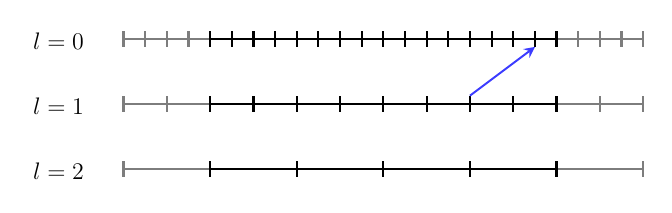
\begin{tikzpicture}[thick,scale=0.275, every node/.style={scale=0.6}]

    % variables
    \def\xl{-8.0}
    \def\xr{8.0}
    \def\y{0.0}
    \def\yy{-3.0}
    \def\yyy{-6.0}
    \def\ts{0.75}
    \def\op{0.35}
    \def\fx{0.15}
    
    % draw ghost cells
    \draw [mygray] (\xl-4,\y+\ts/2) --(\xr+4,\y+\ts/2);
    \draw [mygray] (\xl-4,\yy+\ts/2) --(\xr+4,\yy+\ts/2);
    \draw [mygray] (\xl-4,\yyy+\ts/2) --(\xr+4,\yyy+\ts/2);
    \draw [mygray] (\xl-1.0,\y) --(\xl-1.0,\y+\ts);
    \draw [mygray] (\xr+1.0,\y) --(\xr+1.0,\y+\ts);
    \draw [mygray] (\xl-2.0,\y) --(\xl-2.0,\y+\ts);
    \draw [mygray] (\xr+2.0,\y) --(\xr+2.0,\y+\ts);
    \draw [mygray] (\xl-3.0,\y) --(\xl-3.0,\y+\ts);
    \draw [mygray] (\xr+3.0,\y) --(\xr+3.0,\y+\ts);
    \draw [mygray] (\xl-4.0,\y) --(\xl-4.0,\y+\ts);
    \draw [mygray] (\xr+4.0,\y) --(\xr+4.0,\y+\ts);

    % ghost cells at level l=1
    \draw [mygray] (\xl-2.0,\yy) --(\xl-2.0,\yy+\ts);
    \draw [mygray] (\xr+2.0,\yy) --(\xr+2.0,\yy+\ts);
    \draw [mygray] (\xl-4.0,\yy) --(\xl-4.0,\yy+\ts);
    \draw [mygray] (\xr+4.0,\yy) --(\xr+4.0,\yy+\ts);

    % level l=2
    \draw [mygray] (\xl-4.0,\yyy) --(\xl-4.0,\yyy+\ts);
    \draw [mygray] (\xr+4.0,\yyy) --(\xr+4.0,\yyy+\ts);

    % draw grids
    \draw (\xl,\y+\ts/2) --(\xr,\y+\ts/2);
    \draw (\xl,\yy+\ts/2) --(\xr,\yy+\ts/2);
    \draw (\xl,\yyy+\ts/2) --(\xr,\yyy+\ts/2);
    
    % draw cells for max level
    \draw (\xl,\y) --(\xl,\y+\ts);
    \draw (\xl+1.0,\y) --(\xl+1.0,\y+\ts);
    \draw (\xl+2.0,\y) --(\xl+2.0,\y+\ts);
    \draw (\xl+3.0,\y) --(\xl+3.0,\y+\ts);
    \draw (\xl+4.0,\y) --(\xl+4.0,\y+\ts);
    \draw (\xl+5.0,\y) --(\xl+5.0,\y+\ts);
    \draw (\xl+6.0,\y) --(\xl+6.0,\y+\ts);
    \draw (\xl+7.0,\y) --(\xl+7.0,\y+\ts);
    \draw (\xl+8.0,\y) --(\xl+8.0,\y+\ts);
    \draw (\xl+9.0,\y) --(\xl+9.0,\y+\ts);
    \draw (\xl+10.0,\y) --(\xl+10.0,\y+\ts);
    \draw (\xl+11.0,\y) --(\xl+11.0,\y+\ts);
    \draw (\xl+12.0,\y) --(\xl+12.0,\y+\ts);
    \draw (\xl+13.0,\y) --(\xl+13.0,\y+\ts);
    \draw (\xl+14.0,\y) --(\xl+14.0,\y+\ts);
    \draw (\xl+15.0,\y) --(\xl+15.0,\y+\ts);
    \draw (\xl+16.0,\y) --(\xl+16.0,\y+\ts);
    
    % lower level cells
    \draw (\xl,\yy) --(\xl,\yy+\ts);
    \draw (\xl+2.0,\yy) --(\xl+2.0,\yy+\ts);
    \draw (\xl+4.0,\yy) --(\xl+4.0,\yy+\ts);
    \draw (\xl+6.0,\yy) --(\xl+6.0,\yy+\ts);
    \draw (\xl+8.0,\yy) --(\xl+8.0,\yy+\ts);
    \draw (\xl+10.0,\yy) --(\xl+10.0,\yy+\ts);
    \draw (\xl+12.0,\yy) --(\xl+12.0,\yy+\ts);
    \draw (\xl+14.0,\yy) --(\xl+14.0,\yy+\ts);
    \draw (\xl+16.0,\yy) --(\xl+16.0,\yy+\ts);
    
    % even lower level cells
    \draw (\xl,\yyy) --(\xl,\yyy+\ts);
    \draw (\xl+4.0,\yyy) --(\xl+4.0,\yyy+\ts);
    \draw (\xl+8.0,\yyy) --(\xl+8.0,\yyy+\ts);
    \draw (\xl+12.0,\yyy) --(\xl+12.0,\yyy+\ts);
    \draw (\xl+16.0,\yyy) --(\xl+16.0,\yyy+\ts);
 
    % arrows indicating flux interpolation dependency
    \draw[myblue,->,line width=0.25mm,>=stealth] (\xr-4,\yy+\ts) -- (\xr-1,\y);

    % nodes
    \node at (\xl-7.0,\y+0.25) {\Large $l=0$};
    \node at (\xl-7.0,\yy+0.25) {\Large $l=1$};
    \node at (\xl-7.0,\yyy+0.25) {\Large $l=2$};

\end{tikzpicture}

%        \caption{A block of consisting of $N^{0} = 16$ cells is shown. Four
%        ghost cells are included on each end of the block, allowing the
%        multiresolution decomposition to descend two levels (to grid level
%        $l=2$). Interpolation stencils for the computation of detail
%        coefficients at levels $l=1, l=2$ are shown, indicating the need for ghost cells.}
%    \end{figure}
%    % illustration amr block tree structure
%    \begin{figure}[H]
%        \center
%        \begin{tikzpicture}[sibling distance=2em,every node/.style = {shape=rectangle,align=center,top color=white}]

    % variables
    \def\y{0.0}
    \def\yy{-1.0}
    \def\yyy{-2.0}

    % label levels
    \node at (-2,\y) {$l=1$};
    \node at (-2,\yy) {$l=2$};

    % draw amr blocks
    \draw [thick] (0,\y) rectangle (5,\y);
    \draw [thick] (0,\y-0.1) rectangle (0,\y+0.1);
    \draw [thick] (5,\y-0.1) rectangle (5,\y+0.1);

    \draw [thick] (0,\yy) rectangle (5,\yy);
    \draw [thick] (0,\yy-0.1) rectangle (0,\yy+0.1);
    \draw [thick] (5,\yy-0.1) rectangle (5,\yy+0.1);
    \draw [thick] (2.5,\yy-0.1) rectangle (2.5,\yy+0.1);

    \draw [thick] (2.5,\yyy) rectangle (5,\yyy);
    \draw [thick] (3.75,\yyy-0.1) rectangle (3.75,\yyy+0.1);
    \draw [thick] (2.5,\yyy-0.1) rectangle (2.5,\yyy+0.1);
    \draw [thick] (5,\yyy-0.1) rectangle (5,\yyy+0.1);

    % block labels
    \node [shape=rectangle,align=center] at (2.5,\y) {1};
    \node [shape=rectangle,align=center] at (1.25,\yy) {2};

    % draw tree
    \node at (9,\y) {1}
        child { node {2} }
        child { node {3}[sibling distance=2em,every node/.style = {shape=rectangle,align=center,top color=white}]
            child { node {4} }
            child { node {5} } };

\end{tikzpicture}

%        \caption{}
%    \end{figure}
%
%    % pseudocode of algorithm
%
%    % illustration of parallel issue
%    \begin{figure}[H]
%        \center
%        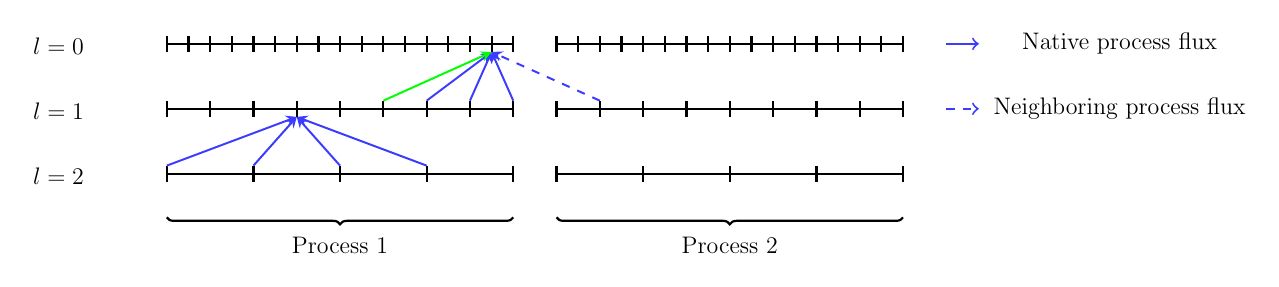
\begin{tikzpicture}[thick,scale=0.275, every node/.style={scale=0.6}]

    % variables
    \def\xl{-8.0}
    \def\xr{8.0}
    \def\y{0.0}
    \def\yy{-3.0}
    \def\yyy{-6.0}
    \def\ts{0.75}
    \def\op{0.35}
    \def\fx{0.15}
    
    % draw grids
    \draw (\xl,\y+\ts/2) --(\xr,\y+\ts/2);
    \draw (\xl,\yy+\ts/2) --(\xr,\yy+\ts/2);
    \draw (\xl,\yyy+\ts/2) --(\xr,\yyy+\ts/2);
    
    % draw cells for max level
    \draw (\xl,\y) --(\xl,\y+\ts);
    \draw (\xl+1.0,\y) --(\xl+1.0,\y+\ts);
    \draw (\xl+2.0,\y) --(\xl+2.0,\y+\ts);
    \draw (\xl+3.0,\y) --(\xl+3.0,\y+\ts);
    \draw (\xl+4.0,\y) --(\xl+4.0,\y+\ts);
    \draw (\xl+5.0,\y) --(\xl+5.0,\y+\ts);
    \draw (\xl+6.0,\y) --(\xl+6.0,\y+\ts);
    \draw (\xl+7.0,\y) --(\xl+7.0,\y+\ts);
    \draw (\xl+8.0,\y) --(\xl+8.0,\y+\ts);
    \draw (\xl+9.0,\y) --(\xl+9.0,\y+\ts);
    \draw (\xl+10.0,\y) --(\xl+10.0,\y+\ts);
    \draw (\xl+11.0,\y) --(\xl+11.0,\y+\ts);
    \draw (\xl+12.0,\y) --(\xl+12.0,\y+\ts);
    \draw (\xl+13.0,\y) --(\xl+13.0,\y+\ts);
    \draw (\xl+14.0,\y) --(\xl+14.0,\y+\ts);
    \draw (\xl+15.0,\y) --(\xl+15.0,\y+\ts);
    \draw (\xl+16.0,\y) --(\xl+16.0,\y+\ts);
    
    % lower level cells
    \draw (\xl,\yy) --(\xl,\yy+\ts);
    \draw (\xl+2.0,\yy) --(\xl+2.0,\yy+\ts);
    \draw (\xl+4.0,\yy) --(\xl+4.0,\yy+\ts);
    \draw (\xl+6.0,\yy) --(\xl+6.0,\yy+\ts);
    \draw (\xl+8.0,\yy) --(\xl+8.0,\yy+\ts);
    \draw (\xl+10.0,\yy) --(\xl+10.0,\yy+\ts);
    \draw (\xl+12.0,\yy) --(\xl+12.0,\yy+\ts);
    \draw (\xl+14.0,\yy) --(\xl+14.0,\yy+\ts);
    \draw (\xl+16.0,\yy) --(\xl+16.0,\yy+\ts);
    
    % even lower level cells
    \draw (\xl,\yyy) --(\xl,\yyy+\ts);
    \draw (\xl+4.0,\yyy) --(\xl+4.0,\yyy+\ts);
    \draw (\xl+8.0,\yyy) --(\xl+8.0,\yyy+\ts);
    \draw (\xl+12.0,\yyy) --(\xl+12.0,\yyy+\ts);
    \draw (\xl+16.0,\yyy) --(\xl+16.0,\yyy+\ts);
    
    % curly brace
    \draw[decoration={brace,mirror,raise=5pt},decorate]
        (\xl,\yyy-1.0) -- node[below=10pt] {\Large Process 1}(\xr,\yyy-1.0);

    % arrows indicating flux interpolation dependency
    \draw[myblue,->,line width=0.25mm,>=stealth] (\xr-4,\yy+\ts) -- (\xr-1,\y);
    \draw[myblue,->,line width=0.25mm,>=stealth] (\xr-2,\yy+\ts) -- (\xr-1,\y);
    \draw[myblue,->,line width=0.25mm,>=stealth] (\xr,\yy+\ts) -- (\xr-1,\y);
    \draw[myblue,dashed,->,line width=0.25mm,>=stealth] (\xr+4,\yy+\ts) -- (\xr-1,\y);
    \draw[green,->,line width=0.25mm,>=stealth] (\xr-6,\yy+\ts) -- (\xr-1,\y);

    \draw[myblue,->,line width=0.25mm,>=stealth] (\xr-16,\yyy+\ts) -- (\xr-10,\yy);
    \draw[myblue,->,line width=0.25mm,>=stealth] (\xr-12,\yyy+\ts) -- (\xr-10,\yy);
    \draw[myblue,->,line width=0.25mm,>=stealth] (\xr-8,\yyy+\ts) -- (\xr-10,\yy);
    \draw[myblue,->,line width=0.25mm,>=stealth] (\xr-4,\yyy+\ts) --(\xr-10,\yy);

    % nodes
    \node at (\xl-5.0,\y+0.25) {\Large $l=0$};
    \node at (\xl-5.0,\yy+0.25) {\Large $l=1$};
    \node at (\xl-5.0,\yyy+0.25) {\Large $l=2$};

    % draw process 2 grid
    \def\xl{10.0}
    \def\xr{26.0}
    \draw (\xl,\y+\ts/2) --(\xr,\y+\ts/2);
    \draw (\xl,\yy+\ts/2) --(\xr,\yy+\ts/2);
    \draw (\xl,\yyy+\ts/2) --(\xr,\yyy+\ts/2);
    
    % draw cells for max level
    \draw (\xl,\y) --(\xl,\y+\ts);
    \draw (\xl+1.0,\y) --(\xl+1.0,\y+\ts);
    \draw (\xl+2.0,\y) --(\xl+2.0,\y+\ts);
    \draw (\xl+3.0,\y) --(\xl+3.0,\y+\ts);
    \draw (\xl+4.0,\y) --(\xl+4.0,\y+\ts);
    \draw (\xl+5.0,\y) --(\xl+5.0,\y+\ts);
    \draw (\xl+6.0,\y) --(\xl+6.0,\y+\ts);
    \draw (\xl+7.0,\y) --(\xl+7.0,\y+\ts);
    \draw (\xl+8.0,\y) --(\xl+8.0,\y+\ts);
    \draw (\xl+9.0,\y) --(\xl+9.0,\y+\ts);
    \draw (\xl+10.0,\y) --(\xl+10.0,\y+\ts);
    \draw (\xl+11.0,\y) --(\xl+11.0,\y+\ts);
    \draw (\xl+12.0,\y) --(\xl+12.0,\y+\ts);
    \draw (\xl+13.0,\y) --(\xl+13.0,\y+\ts);
    \draw (\xl+14.0,\y) --(\xl+14.0,\y+\ts);
    \draw (\xl+15.0,\y) --(\xl+15.0,\y+\ts);
    \draw (\xl+16.0,\y) --(\xl+16.0,\y+\ts);
    
    % lower level cells
    \draw (\xl,\yy) --(\xl,\yy+\ts);
    \draw (\xl+2.0,\yy) --(\xl+2.0,\yy+\ts);
    \draw (\xl+4.0,\yy) --(\xl+4.0,\yy+\ts);
    \draw (\xl+6.0,\yy) --(\xl+6.0,\yy+\ts);
    \draw (\xl+8.0,\yy) --(\xl+8.0,\yy+\ts);
    \draw (\xl+10.0,\yy) --(\xl+10.0,\yy+\ts);
    \draw (\xl+12.0,\yy) --(\xl+12.0,\yy+\ts);
    \draw (\xl+14.0,\yy) --(\xl+14.0,\yy+\ts);
    \draw (\xl+16.0,\yy) --(\xl+16.0,\yy+\ts);
    
    % even lower level cells
    \draw (\xl,\yyy) --(\xl,\yyy+\ts);
    \draw (\xl+4.0,\yyy) --(\xl+4.0,\yyy+\ts);
    \draw (\xl+8.0,\yyy) --(\xl+8.0,\yyy+\ts);
    \draw (\xl+12.0,\yyy) --(\xl+12.0,\yyy+\ts);
    \draw (\xl+16.0,\yyy) --(\xl+16.0,\yyy+\ts);
    
    % curly brace
    \draw[decoration={brace,mirror,raise=5pt},decorate]
        (\xl,\yyy-1.0) -- node[below=10pt] {\Large Process 2}(\xr,\yyy-1.0);

    % legend
    \draw[myblue,->,line width=0.25mm] (\xr+2,\y+\ts/2) -- (\xr+3.5,\y+\ts/2);
    \draw[myblue,->,dashed,line width=0.25mm] (\xr+2,\yy+\ts/2) -- (\xr+3.5,\yy+\ts/2);
    \node at (\xr+10,\y+\ts/2) {\Large Native process flux};
    \node at (\xr+10,\yy+\ts/2) {\Large Neighboring process flux};

\end{tikzpicture}

%       \caption{Two examples of flux interpolation on a hierarchy of grids
%        on Process 1: one procedure requires flux data from the adjacent
%        process, the other does not.}
%    \end{figure}
%
%    \subsection*{Buffer Region}
%
%    \subsection*{Load Balancing}

\section{Numerical Results}

    \subsection*{Interacting blast waves}

        % problem description
        The adaptive multiresolution scheme is tested for the problem of two
        interacting blast waves (cite collela woodward).  We solve the Euler
        equations in one spatial dimension,

%        \begin{equation}
%           u_{t} + f(u)_{x} = 0,
%        \label{euler1d}
%        \end{equation}
%        where
%        \begin{equation}
%            u =
%            \begin{pmatrix}
%                \rho \\ \rho u \\ E
%            \end{pmatrix}, \quad
%            f =
%            \begin{pmatrix}
%                \rho u \\ \rho u^2 + p \\ u( E + p )
%            \end{pmatrix},
%        \end{equation}
%        and the total energy per unit volume is given by
%        \begin{equation*}
%            E = \rho \left( \frac{1}{2} u^2 + e \right).
%        \end{equation*}

%        % convergence rates table (epsilon shouldn't be below error of scheme)
%        % note: include estimated order of error of reference scheme)
%        \begin{center}\vspace{1cm}
%        \begin{tabular}{|l|l|l|l|l|l|l|l|l|}
%        \hline
%                   & \multicolumn{4}{l|}{$\varepsilon = 0.0$}              & \multicolumn{4}{l|}{$\varepsilon = 10^{-12}$}         \\ \hline
%        grid cells & $L_{1}$ error & order & $L_{\infty}$ error & order & $L_{1}$ error & order & $L_{\infty}$ error & order \\ \hline
%        16         &               &       &                    &       &               &       &                    &       \\ \hline
%        32         &               &       &                    &       &               &       &                    &       \\ \hline
%        64         &               &       &                    &       &               &       &                    &       \\ \hline
%        128        &               &       &                    &       &               &       &                    &       \\ \hline
%        256        &               &       &                    &       &               &       &                    &       \\ \hline
%                   & \multicolumn{4}{l|}{$\varepsilon = 10^{-6}$}          & \multicolumn{4}{l|}{$\varepsilon = 10^{-4}$}          \\ \hline
%        grid cells & $L_{1}$ error & order & $L_{\infty}$ error & order & $L_{1}$ error & order & $L_{\infty}$ error & order \\ \hline
%        16         &               &       &                    &       &               &       &                    &       \\ \hline
%        32         &               &       &                    &       &               &       &                    &       \\ \hline
%        64         &               &       &                    &       &               &       &                    &       \\ \hline
%        128        &               &       &                    &       &               &       &                    &       \\ \hline
%        256        &               &       &                    &       &               &       &                    &       \\ \hline
%        \end{tabular}
%        \end{center}\vspace{1cm}

    \subsection*{Mach reflection}

    \subsection*{Nuclear burning}


%        % problem description
%        Using the inviscid flow assumption, the dynamics of compressible fluids are
%        modeled using the reactive Euler equations \hl{add domain notation}
%        \begin{equation}
%           u_{t} + f(u)_{x}
%           + g(u)_{y} = s(u),
%            \label{goveq}
%        \end{equation}
%        where $u = \left( \rho, \rho u, \rho v, \rho w, E \right)^{T}$ is
%        the state vector, the flux vectors are given by
%        \begin{equation}
%            f = 
%        \begin{pmatrix}
%        \rho u \\ \rho u^2 + p \\ \rho u v \\ u( E + p )
%        \end{pmatrix}, \text{ } \text{ } \text{ }
%            g = 
%        \begin{pmatrix}
%        \rho v \\ \rho u v \\ \rho v^2 + p \\ v( E + p )
%        \end{pmatrix},
%        \end{equation}
%        and $s(u)$ represents sources. The total energy per
%        unit volume is given by
%        \begin{equation*}
%            E = \rho \left( \frac{1}{2} \mathbf{V}^{2} + e \right),
%        \end{equation*}
%        where $e$ is the internal energy and the kinetic energy contribution is
%        \begin{equation*}
%            \frac{1}{2} \mathbf{V}^{2} = \frac{1}{2} \mathbf{V}
%            \cdot \mathbf{V} = \frac{1}{2} \left( u^2 + v^2 \right).
%        \end{equation*}
%        The system of nonlinear equations is closed by an
%        equation of state which is in general not derived from that of an ideal gas.

\appendix
%\section{Multiresolution Analysis}
%
%    % describe multiresolution analysis (sourced from tymczak2000)
%    A multiresolution analysis (MRA) of the Lebesgue space
%    $L^{2}(\mathbb{R})$ defines a sequence of nested approximation spaces.
%    These spaces satisfy certain self-similarity properties in both space
%    and scale. An MRA defines a sequence of closed subspaces $\{ \mathcal{V}_{j} : j \in
%    \mathbb{Z} \}$ such that
%    \begin{equation*}
%        \mathcal{V}_{0} \subset \mathcal{V}_{1} \subset \mathcal{V}_{2} \subset \cdots
%        \subset L^{2}.
%    \end{equation*}
%    The complement of $\mathcal{V}_{j} \in \mathcal{V}_{j+1}$ is defined by
%    $\mathcal{W}_{j}$, known as the detail space. This relation is defined
%    by a direct summation as
%    \begin{equation*}
%        \mathcal{V}_{j+1} = \mathcal{W}_{j} \oplus \mathcal{V}_{j}.
%    \end{equation*}
%    Considering successively finer approximation spaces yields for any
%    arbitrary level $J$,
%    \begin{equation*}
%        \mathcal{V}_{J} = \mathcal{V}_0 \oplus \mathcal{W}_0 \oplus \mathcal{W}_1 \oplus \dots \oplus \mathcal{W}_{J-1}.
%    \end{equation*}
%    Thus fine-scale information on any arbitrary level $J$ is represented by
%    the coarsest scale plus a series of differences at higher levels.
%    Interested readers can refer to (\hl{cite}) for more details on the
%    construction of the bi-orthogonal multiresolution analysis used.
%
%    %, a real-valued scaling function
%    %$\phi_{j}(x) \in V_{j}$ is defined which forms a basis,
%    %\begin{equation*}
%    %    V_{j} = \text{span} \left\{ \phi_{j}(x+k) : \forall k \right\}.
%    %\end{equation*}
%

\section{Derivation of Prediction Operator in One-Dimension}

    % derivation of prediction operator
    We are interested in obtaining the difference between approximation spaces at varying levels of resolution. We 
    are given cell-averaged values as input data to our wavelet transform. This data is fed to the scheme at some arbitrary maximum
    resolution level $J$, and the wavelet transform produces details coefficients at each lower level until the coarsest level,
    $j=0$, is reached. The coefficients in this case are interchangeable with the cell-averages and are denoted by $u^{j}_{k}$,
    where the level of resolution is denoted by $j$, and the spatial index is denoted by $k$. We consider an interpolating
    polynomial $p(x)$ such that 
    \begin{align}
        u^{j}_{k-1} &= \int_{x^{j}_{k-1}}^{x^{j}_{k}} p(x) dx \\
        u^{j}_{k} &= \int_{x^{j}_{k}}^{x^{j}_{k+1}} p(x) dx \\
        u^{j}_{k+1} &= \int_{x^{j}_{k+1}}^{x^{j}_{k+2}} p(x) dx.
    \end{align}
    The polynomial $p(x)$ should then predict the finer cell-averages of cell $u^{j}_{k}$ as
    \begin{align}
        \tilde{u}^{j+1}_{2k} &= 2 \int_{x^{j}_{k}}^{x^{j}_{k+1/2}} p(x) dx \\
        \tilde{u}^{j+1}_{2k+1} &= 2 \int_{x^{j}_{k+1/2}}^{x^{j}_{k+1}} p(x) dx
    \end{align}
    At present, it may not be clear how to implement such a scheme on a computer. However this interpolation procedure
    can be cast in a more suitable form by introducing another polynomial, the integral of $p(x)$:
    \begin{equation}
        P(x) = \int_{0}^{x} p(y) dy.
    \end{equation}
    Now the problem is to interpolate the following data
    \begin{align}
        0 &= P(x^{j}_{k-1}) \\
        u^{j}_{k-1} &= P(x^{j}_{k}) \\
        u^{j}_{k-1} + u^{j}_{k} &= P(x^{j}_{k+1}) \\
        u^{j}_{k-1} + u^{j}_{k} + u^{j}_{k+1} &= P(x^{j}_{k+2}).
    \end{align}
    This can easily be done using Lagrange polynomials. Then the predictions are given in terms of $P(x)$ by
    \begin{align}
        \tilde{u}^{j+1}_{2k} &= 2 \left( P(x^{j}_{k+1/2}) - P(x^{j}_{k}) \right) \\
        \tilde{u}^{j+1}_{2k+1} &= 2 \left( P(x^{j}_{k+1}) - P(x^{j}_{k+1/2}) \right).
    \end{align}
    This interpolating polynomial is cast in the Lagrange form,
    \begin{equation}
    P(x) = \sum_{i=0}^{n} y_{i} l_{i}(x),
    \end{equation}
    where $y_{i}$ are the functional data, and $l_{i}(x)$ are the Lagrange polynomials. For $n=3$ these
    are given by
    \begin{align}
        l_{0}(x) &= \frac{x-x_1}{x_0-x_1} \frac{x-x_2}{x_0-x_2} \frac{x-x_3}{x_0-x_3} \\
        l_{1}(x) &= \frac{x-x_0}{x_1-x_0} \frac{x-x_2}{x_1-x_2} \frac{x-x_3}{x_1-x_3} \\
        l_{2}(x) &= \frac{x-x_0}{x_2-x_0} \frac{x-x_1}{x_2-x_1} \frac{x-x_3}{x_2-x_3} \\
        l_{3}(x) &= \frac{x-x_0}{x_3-x_0} \frac{x-x_1}{x_3-x_1} \frac{x-x_2}{x_3-x_2},
    \end{align}
    and the final interpolating polynomial is
    \begin{equation}
        P(x) = (0) l_{0}(x) + ( u^{j}_{k-1} ) l_{1}(x) + ( u^{j}_{k-1} + u^{j}_{k} ) l_{2}(x)
            + ( u^{j}_{k-1} + u^{j}_{k} + u^{j}_{k+1} ) l_{3}(x).
    \end{equation}
    Several evaluations are necessary in order to obtain the predictions. Using intervals of equal length, these values are
    \begin{align}
        P(x^{j}_{k}) &= u^{j}_{k-1} \\
        P(x^{j}_{k+1/2}) &= \frac{17}{16} u^{j}_{k-1} + \frac{1}{2} u^{j}_{k} - \frac{1}{16} u^{j}_{k+1} \\
        P(x^{j}_{k+1}) &= u^{j}_{k-1} + u^{j}_{k}.
    \end{align}
    Then the predictions of the cell-averages at the higher level of resolution are finally given by
    \begin{align}
        \tilde{u}^{j+1}_{2k} & = u^{j}_{k} + \frac{1}{8} \left( u^{j}_{k-1} - u^{j}_{k+1} \right) \\
        \tilde{u}^{j+1}_{2k+1} & = u^{j}_{k} - \frac{1}{8} \left( u^{j}_{k-1} - u^{j}_{k+1} \right).
    \end{align}
    This procedure could easily be extended to non-uniformly spaced intervals,
    giving different weights.
    \begin{table}
        \center
        \begin{tabular}{|l|l|l|l|}
        \hline
            order    & $\gamma_{1}$ & $\gamma_{2}$ & $\gamma_{3}$ \\ \hline
            3 & -1/8          & 0            & 0            \\ \hline
            5 & -22/128      & 3/128        & 0            \\ \hline
            7 & 0            & 0            & 0            \\ \hline
        \end{tabular}
        \label{coeff1}
        \caption{Coefficients for centered, conservative interpolants of orders 3-7.}
    \end{table}
    \begin{align}
        \tilde{u}^{j+1}_{2k+1} & = \frac{5}{8} u^{j}_{k}
        + \frac{1}{2} u^{j}_{k+1} - \frac{1}{8} u^{j}_{k+2} \\
        \tilde{u}^{j+1}_{2k+1} & = \frac{1}{8} u^{j}_{k-2}
        - \frac{1}{2} u^{j}_{k-1} + \frac{11}{8} u^{j}_{k}.
    \end{align}
    \begin{table}[]
        \center
        \begin{tabular}{|l|l|l|l|l|}
        \hline
            order    & $\beta_{1}$ & $\beta_{2}$ & $\beta_{3}$ & $\beta_{4}$ \\ \hline
            4 & 9/16         & -1/16        & 0            & 0 \\ \hline
            6 & 75/128       & -25/256      & 3/256        & 0 \\ \hline
            8 & 1225/2048    & -245/2048    & 49/2048      & -5/2048 \\ \hline
        \end{tabular}
        \label{coeff2}
        \caption{Coefficients for centered, point-wise interpolation of orders 4-8}
    \end{table}

    \section{WENO Reconstruction}

        % Idea: Is it possible to do the multiresolution transform using WENO
        % prediction operators?

        % describe the dang weno
        The class of WENO schemes are designed to provide the smoothest
        polynomial for reconstructing the solution field. In the following work,
        we utilize the recent hierarchical WENO schemes of Zhu et. al.,
        \cite{zhu2018}. We briefly review the fundamentals of the approach in
        this section.

        To provide left and right states as input to the Rieman solver, the
        final WENO polynomial is evaluated at cell interfaces, $u(x_{i\pm1/2})$.
        Given a target cell $I_{i}$, we first construct polynomials $q_{s}(x)$
        of degree $2s$ based on the stencils $\mathcal{T}_{s} = \left\{ I_{i-s},
        \dots, I_{i+s} \right\}$, which preserve respective cell averages.  The
        polynomial $q(x)$ is evaluated at interfaces $x_{i-1/2}$ and $x_{i+1/2}$
        to provide the states $u_{i-1/2}^{R}$ and $u_{i+1/2}^{L}$, respectively.
        The result of the polynomials evaluated at the interface $x_{i+1/2}$ are
        \begin{equation}
            q_{s}(x_{i+1/2}) = \sum_{j \in \mathcal{T}_{s}} \alpha_{s,j} u_{j},
        \end{equation}
        where the weights $\alpha_{s,j}$ are provided in Table(\ref{coeff3}).
        Evaluating the polynomial at the interface $x_{i-1/2}$ is
        mirror-symmetric about the target cell. \\

        The next step is to construct polynomials $p_{s}(x)$ using a convex
        combination of the $q_{s}(x)$. We have
        \begin{equation}
            p_{s}(x) = \frac{1}{\gamma_{s,s}} q_{s}(x) - \sum_{l=1}^{s-1}
            \frac{\gamma_{l,s}}{\gamma_{s,s}} p_{l}(x),
        \end{equation}
        where the linear weights $\gamma$ are supplied in Table (\hl{ref}). \\

        Smoothness indicators are used to determine the near-optimal weight to
        ascribe to each of the candidate polynomials, $p_{s}(x)$. We use the
        same indicator and nonlinear weights as in (\cite{zhu2018},\hl{others}).
        The final polynomial reconstruction is 
        \begin{equation}
            w_{s}(x) = \sum_{l=1}^{s} \omega_{l,s} p_{l}(x).
        \end{equation}
 
        \begin{table}[H]
            \center
            \begin{tabular}{|l|l|l|l|l|l|l|l|l|l|}
            \hline
                order & $\alpha_{i-4}$ & $\alpha_{i-3}$ & $\alpha_{i-2}$ &
                $\alpha_{i-1}$ & $\alpha_{i}$ & $\alpha_{i+1}$ & $\alpha_{i+2}$
                & $\alpha_{i+3}$ & $\alpha_{i+4}$ \\ \hline
                3 & 0 & 0 & 0 & -1/6 & 5/6 & 1/3 & 0 & 0 & 0 \\ \hline
                5 & 0 & 0 & 1/30 & -13/60 & 47/60 & 9/20 & -1/20 & 0 & 0 \\ \hline
                7 & 0 & 0 & 0 & 0 & 0 & 0 & 0 & 0 & 0 \\ \hline
                9 & 0 & 0 & 0 & 0 & 0 & 0 & 0 & 0 & 0 \\ \hline
            \end{tabular}
            \label{coeff3}
            \caption{}
        \end{table}

    \begin{thebibliography}{9}

        \bibitem{harten1994}
        Harten, A.,
        Adaptive Multiresolution Schemes for Shock Computations,
        Journal of Computational Physics,
        Volume 115, pg 319-338
        1994.

        \bibitem{woodward1984}
        Woodward, P. and Colella, P.,
        The Numerical Simulation of Two-Dimensional Fluid Flow with Strong Shocks,
        Journal of Computational Physics,
        Volume 54, pg 115-173
        1984.

        \bibitem{bihari1999}
	    Bihari, B.L., and Schwendeman, D.,
	    Multiresolution Schemes for the Reactive Euler Equations,
	    Journal of Computational Physics,
        Volume 154, pg 197-230
        1999.

        \bibitem{shu2009}
        Shu, Chi-Wang,
        High Order Weighted Essentially Nonoscillatory Schemes for Convection Dominated Problems,
        SIAM Review,
        Volume 51, pg 82-126.

        \bibitem{zhu2018}
        Zhu, and Shu, Chi-Wang,
        A new type of multi-resolution WENO schemes with increasingly higher order of accuracy,
        Unknown,
        Unknown,
        2018.





    \end{thebibliography}

\end{document}

